%**************************************************************************
%*
%*  Instrucciones para la platilla del informe final
%*
%*  
%*
%*  Filename: platillapaper.tex
%*
%*
%*  
%*  
%*
%**************************************************************************


\documentclass{wscpaperproc}
\usepackage[spanish]{babel}
\usepackage{latexsym}
\usepackage{caption}
\usepackage{csquotes}
\usepackage{graphicx}
\usepackage{mathptmx}
\usepackage{pgf}
\usepackage[T1]{fontenc}
\usepackage[style=numeric,backend=biber,defernumbers=true]{biblatex}
\addbibresource{EDO Final Work.bib}

%
%****************************************************************************
% AUTHOR: You may want to use some of these packages. (Optional)
\usepackage{amsmath}
\usepackage{amsfonts}
\usepackage{amssymb}
\usepackage{amsbsy}
\usepackage{amsthm}
\usepackage{pgf}
\usepackage{subcaption}
\usepackage[colorlinks=true,urlcolor=blue,citecolor=black,anchorcolor=black,linkcolor=red]{hyperref}
\usepackage{hyperref}
%****************************************************************************


%
%****************************************************************************
% AUTHOR: If you do not wish to use hyperlinks, then just comment
% out the hyperref usepackage commands below.

%% This version of the command is used if you use pdflatex. In this case you
%% cannot use ps or eps files for graphics, but pdf, jpeg, png etc are fine.

%% The next versions of the hyperref command are used if you adopt the
%% outdated latex-dvips-ps2pdf route in generating your pdf file. In
%% this case you can use ps or eps files for graphics, but not pdf, jpeg, png etc.
%% However, the final pdf file should embed all fonts required which means that you have to use file
%% formats which can embed fonts. Please note that the final PDF file will not be generated on your computer!
%% If you are using WinEdt or PCTeX, then use the following. If you are using
%% Y&Y TeX then replace "dvips" with "dvipsone"

%%\usepackage[dvips,colorlinks=true,urlcolor=blue,citecolor=black,%
%% anchorcolor=black,linkcolor=black]{hyperref}
%****************************************************************************


%
%****************************************************************************
%*
%* AUTHOR: YOUR CALL!  Document-specific macros can come here.
%*
%****************************************************************************

% If you use theoremes
\newtheoremstyle{wsc}% hnamei
{3pt}% hSpace abovei
{3pt}% hSpace belowi
{}% hBody fonti
{}% hIndent amounti1
{\bf}% hTheorem head fontbf
{}% hPunctuation after theorem headi
{.5em}% hSpace after theorem headi2
{}% hTheorem head spec (can be left empty, meaning `normal')i

\theoremstyle{wsc}
\newtheorem{theorem}{Teorema}
\renewcommand{\thetheorem}{\arabic{theorem}}
\newtheorem{corollary}[theorem]{Corolario}
\renewcommand{\thecorollary}{\arabic{corollary}}
\newtheorem{definition}{Definici\'on}
\renewcommand{\thedefinition}{\arabic{definition}}


%#########################################################
%*
%*  The Document.
%*
\begin{document}

%***************************************************************************
% AUTHOR: AUTHOR NAMES GO HERE
% FORMAT AUTHORS NAMES Like: Author1, Author2 and Author3 (last names)
%
%		You need to change the author listing below!
%               Please list ALL authors using last name only, separate by a comma except
%               for the last author, separate with "and"
%
\WSCpagesetup{Machado, Toledo, Moreno, Concepci\'on, Navarro}

% AUTHOR: Enter the title, all letters in upper case
\title{Estabilidad y simulaci\'on num\'erica del sistema presa-depredador con respuestas funcionales de tipo II de Holling para presas adultas}

% AUTHOR: Enter the authors of the article, see end of the example document for further examples
\author{
	Daniel Machado \\[12pt]
	Grupo C211\\
	Ciencia de la Computaci\'on\\
	Facultad de Matem\'atica y Computaci\'on\\
	Universidad de La Habana. Cuba\\
	% Multiple authors are entered as follows.
	% You may also need to adjust the titlevbox size in the preamble - search for titlevboxsize
	\and
	Daniel Toledo\\[12pt]
	Grupo C211\\
	Ciencia de la Computaci\'on\\
	Facultad de Matem\'atica y Computaci\'on\\
	Universidad de La Habana. Cuba\\
	\and
	Osvaldo Moreno\\[12pt]
	Grupo C211\\
	Ciencia de la Computaci\'on\\
	Facultad de Matem\'atica y Computaci\'on\\
	Universidad de La Habana. Cuba\\
	\and
	Jos\'e Antonio Concepci\'on\\[12pt]
	Grupo C211\\
	Ciencia de la Computaci\'on\\
	Facultad de Matem\'atica y Computaci\'on\\
	Universidad de La Habana. Cuba\\
	\and
	Adri\'an Navarro\\[12pt]
	Grupo C211\\
	Ciencia de la Computaci\'on\\
	Facultad de Matem\'atica y Computaci\'on\\
	Universidad de La Habana. Cuba\\
}



\maketitle

\section*{Resumen}
Este documento presenta un análisis local exhaustivo del modelo depredador-presa con estructura de
etapas en la población de presa y respuestas funcionales de Holling de tipo II y I \cite{holling_functional_1965}. Los autores determinan
los tres posibles equilibrios, analizan la estabilidad local a través de la matriz jacobiana, realizan
simulaciones numéricas y obtienen varios resultados clave. El equilibrio trivial siempre es inestable,
el equilibrio con predadores extintos es estable bajo ciertas condiciones y el equilibrio interior puede
ser estable o inestable dependiendo de los parámetros. Las simulaciones numéricas corroboran estos resultados
y muestran cómo las poblaciones evolucionan hacia uno de los tres puntos de equilibrio dependiendo de las
condiciones iniciales y los valores de parámetros.

\section{INTRODUCCI\'ON}
\label{sec:intro}
El artículo titulado "Local Analysis of the Prey-Predator Model with Stage-Structure Prey and Holling
Type Functional Responses" por Dian Savitri fue publicado en 2019
en el Journal of Physics: Conference Series. Su factor de impacto tiene una puntuaci\'on de 0.21 en el
período 2022-2023. El artículo analiza el modelo depredador-presa con dos tipos de presa en estructura
de etapas y un solo depredador. La población de presas se divide en adultos y juveniles. El depredador
exhibe diferentes tasas de depredación para adultos e inmaduros. Se utilizan respuestas funcionales de
Holling tipo II \cite{holling_functional_1965} para adultos y tipo I para juveniles. El estudio tuvo los siguientes objetivos:
determinar los puntos de equilibrio del modelo, analizar la estabilidad local de los puntos de equilibrio
utilizando la matriz jacobiaana y autovalores y observar el comportamiento dinámico del modelo mediante
simulaciones numéricas y diagramas de fase. Además utilizaron las siguientes técnicas para obtener resultados
más rigurosos: análisis matemático para determinar los puntos de equilibrio y condiciones de estabilidad,
cálculo de la matriz jacobiana y autovalores en cada punto de equilibrio, aplicación del Criterio de Routh-Hurwitz
para analizar la estabilidad del equilibrio interior, simulaciones numéricas utilizando el método Runge-Kutta de
cuarto orden y un análisis de bifurcación para estudiar la posible existencia de ciclos límite. (no estoy seguro de esta traduccion revisar despues)
\subsection{Estructura del trabajo}

\begin{figure}[h]
	\centering
	\begin{subfigure}[b]{0.5\textwidth}
		\centering
		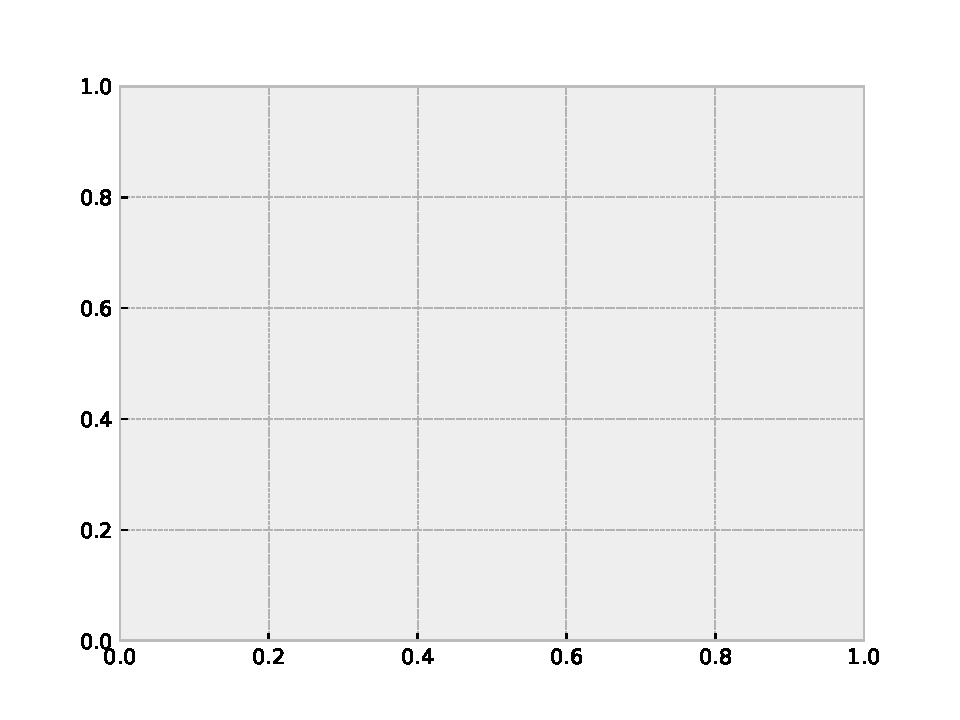
\includegraphics[width=\textwidth]{Plotting.pdf}
		\caption{Gráfica en formato PDF}
		\label{fig:grafica1}
	\end{subfigure}%
	\begin{subfigure}[b]{0.5\textwidth}
		\centering
		\resizebox{\textwidth}{!}{%% Creator: Matplotlib, PGF backend
%%
%% To include the figure in your LaTeX document, write
%%   \input{<filename>.pgf}
%%
%% Make sure the required packages are loaded in your preamble
%%   \usepackage{pgf}
%%
%% Also ensure that all the required font packages are loaded; for instance,
%% the lmodern package is sometimes necessary when using math font.
%%   \usepackage{lmodern}
%%
%% Figures using additional raster images can only be included by \input if
%% they are in the same directory as the main LaTeX file. For loading figures
%% from other directories you can use the `import` package
%%   \usepackage{import}
%%
%% and then include the figures with
%%   \import{<path to file>}{<filename>.pgf}
%%
%% Matplotlib used the following preamble
%%   \usepackage{fontspec}
%%   \setmainfont{DejaVuSerif.ttf}[Path=\detokenize{/usr/share/matplotlib/mpl-data/fonts/ttf/}]
%%   \setsansfont{DejaVuSans.ttf}[Path=\detokenize{/usr/share/matplotlib/mpl-data/fonts/ttf/}]
%%   \setmonofont{DejaVuSansMono.ttf}[Path=\detokenize{/usr/share/matplotlib/mpl-data/fonts/ttf/}]
%%
\begingroup%
\makeatletter%
\begin{pgfpicture}%
\pgfpathrectangle{\pgfpointorigin}{\pgfqpoint{6.400000in}{4.800000in}}%
\pgfusepath{use as bounding box, clip}%
\begin{pgfscope}%
\pgfsetbuttcap%
\pgfsetmiterjoin%
\definecolor{currentfill}{rgb}{1.000000,1.000000,1.000000}%
\pgfsetfillcolor{currentfill}%
\pgfsetlinewidth{0.000000pt}%
\definecolor{currentstroke}{rgb}{1.000000,1.000000,1.000000}%
\pgfsetstrokecolor{currentstroke}%
\pgfsetdash{}{0pt}%
\pgfpathmoveto{\pgfqpoint{0.000000in}{0.000000in}}%
\pgfpathlineto{\pgfqpoint{6.400000in}{0.000000in}}%
\pgfpathlineto{\pgfqpoint{6.400000in}{4.800000in}}%
\pgfpathlineto{\pgfqpoint{0.000000in}{4.800000in}}%
\pgfpathlineto{\pgfqpoint{0.000000in}{0.000000in}}%
\pgfpathclose%
\pgfusepath{fill}%
\end{pgfscope}%
\begin{pgfscope}%
\pgfsetbuttcap%
\pgfsetmiterjoin%
\definecolor{currentfill}{rgb}{0.933333,0.933333,0.933333}%
\pgfsetfillcolor{currentfill}%
\pgfsetlinewidth{0.000000pt}%
\definecolor{currentstroke}{rgb}{0.000000,0.000000,0.000000}%
\pgfsetstrokecolor{currentstroke}%
\pgfsetstrokeopacity{0.000000}%
\pgfsetdash{}{0pt}%
\pgfpathmoveto{\pgfqpoint{0.800000in}{0.528000in}}%
\pgfpathlineto{\pgfqpoint{5.760000in}{0.528000in}}%
\pgfpathlineto{\pgfqpoint{5.760000in}{4.224000in}}%
\pgfpathlineto{\pgfqpoint{0.800000in}{4.224000in}}%
\pgfpathlineto{\pgfqpoint{0.800000in}{0.528000in}}%
\pgfpathclose%
\pgfusepath{fill}%
\end{pgfscope}%
\begin{pgfscope}%
\pgfpathrectangle{\pgfqpoint{0.800000in}{0.528000in}}{\pgfqpoint{4.960000in}{3.696000in}}%
\pgfusepath{clip}%
\pgfsetbuttcap%
\pgfsetroundjoin%
\pgfsetlinewidth{0.501875pt}%
\definecolor{currentstroke}{rgb}{0.698039,0.698039,0.698039}%
\pgfsetstrokecolor{currentstroke}%
\pgfsetdash{{1.850000pt}{0.800000pt}}{0.000000pt}%
\pgfpathmoveto{\pgfqpoint{1.025455in}{0.528000in}}%
\pgfpathlineto{\pgfqpoint{1.025455in}{4.224000in}}%
\pgfusepath{stroke}%
\end{pgfscope}%
\begin{pgfscope}%
\pgfsetbuttcap%
\pgfsetroundjoin%
\definecolor{currentfill}{rgb}{0.000000,0.000000,0.000000}%
\pgfsetfillcolor{currentfill}%
\pgfsetlinewidth{0.803000pt}%
\definecolor{currentstroke}{rgb}{0.000000,0.000000,0.000000}%
\pgfsetstrokecolor{currentstroke}%
\pgfsetdash{}{0pt}%
\pgfsys@defobject{currentmarker}{\pgfqpoint{0.000000in}{0.000000in}}{\pgfqpoint{0.000000in}{0.048611in}}{%
\pgfpathmoveto{\pgfqpoint{0.000000in}{0.000000in}}%
\pgfpathlineto{\pgfqpoint{0.000000in}{0.048611in}}%
\pgfusepath{stroke,fill}%
}%
\begin{pgfscope}%
\pgfsys@transformshift{1.025455in}{0.528000in}%
\pgfsys@useobject{currentmarker}{}%
\end{pgfscope}%
\end{pgfscope}%
\begin{pgfscope}%
\definecolor{textcolor}{rgb}{0.000000,0.000000,0.000000}%
\pgfsetstrokecolor{textcolor}%
\pgfsetfillcolor{textcolor}%
\pgftext[x=1.025455in,y=0.479389in,,top]{\color{textcolor}\sffamily\fontsize{10.000000}{12.000000}\selectfont 0}%
\end{pgfscope}%
\begin{pgfscope}%
\pgfpathrectangle{\pgfqpoint{0.800000in}{0.528000in}}{\pgfqpoint{4.960000in}{3.696000in}}%
\pgfusepath{clip}%
\pgfsetbuttcap%
\pgfsetroundjoin%
\pgfsetlinewidth{0.501875pt}%
\definecolor{currentstroke}{rgb}{0.698039,0.698039,0.698039}%
\pgfsetstrokecolor{currentstroke}%
\pgfsetdash{{1.850000pt}{0.800000pt}}{0.000000pt}%
\pgfpathmoveto{\pgfqpoint{1.929080in}{0.528000in}}%
\pgfpathlineto{\pgfqpoint{1.929080in}{4.224000in}}%
\pgfusepath{stroke}%
\end{pgfscope}%
\begin{pgfscope}%
\pgfsetbuttcap%
\pgfsetroundjoin%
\definecolor{currentfill}{rgb}{0.000000,0.000000,0.000000}%
\pgfsetfillcolor{currentfill}%
\pgfsetlinewidth{0.803000pt}%
\definecolor{currentstroke}{rgb}{0.000000,0.000000,0.000000}%
\pgfsetstrokecolor{currentstroke}%
\pgfsetdash{}{0pt}%
\pgfsys@defobject{currentmarker}{\pgfqpoint{0.000000in}{0.000000in}}{\pgfqpoint{0.000000in}{0.048611in}}{%
\pgfpathmoveto{\pgfqpoint{0.000000in}{0.000000in}}%
\pgfpathlineto{\pgfqpoint{0.000000in}{0.048611in}}%
\pgfusepath{stroke,fill}%
}%
\begin{pgfscope}%
\pgfsys@transformshift{1.929080in}{0.528000in}%
\pgfsys@useobject{currentmarker}{}%
\end{pgfscope}%
\end{pgfscope}%
\begin{pgfscope}%
\definecolor{textcolor}{rgb}{0.000000,0.000000,0.000000}%
\pgfsetstrokecolor{textcolor}%
\pgfsetfillcolor{textcolor}%
\pgftext[x=1.929080in,y=0.479389in,,top]{\color{textcolor}\sffamily\fontsize{10.000000}{12.000000}\selectfont 1}%
\end{pgfscope}%
\begin{pgfscope}%
\pgfpathrectangle{\pgfqpoint{0.800000in}{0.528000in}}{\pgfqpoint{4.960000in}{3.696000in}}%
\pgfusepath{clip}%
\pgfsetbuttcap%
\pgfsetroundjoin%
\pgfsetlinewidth{0.501875pt}%
\definecolor{currentstroke}{rgb}{0.698039,0.698039,0.698039}%
\pgfsetstrokecolor{currentstroke}%
\pgfsetdash{{1.850000pt}{0.800000pt}}{0.000000pt}%
\pgfpathmoveto{\pgfqpoint{2.832705in}{0.528000in}}%
\pgfpathlineto{\pgfqpoint{2.832705in}{4.224000in}}%
\pgfusepath{stroke}%
\end{pgfscope}%
\begin{pgfscope}%
\pgfsetbuttcap%
\pgfsetroundjoin%
\definecolor{currentfill}{rgb}{0.000000,0.000000,0.000000}%
\pgfsetfillcolor{currentfill}%
\pgfsetlinewidth{0.803000pt}%
\definecolor{currentstroke}{rgb}{0.000000,0.000000,0.000000}%
\pgfsetstrokecolor{currentstroke}%
\pgfsetdash{}{0pt}%
\pgfsys@defobject{currentmarker}{\pgfqpoint{0.000000in}{0.000000in}}{\pgfqpoint{0.000000in}{0.048611in}}{%
\pgfpathmoveto{\pgfqpoint{0.000000in}{0.000000in}}%
\pgfpathlineto{\pgfqpoint{0.000000in}{0.048611in}}%
\pgfusepath{stroke,fill}%
}%
\begin{pgfscope}%
\pgfsys@transformshift{2.832705in}{0.528000in}%
\pgfsys@useobject{currentmarker}{}%
\end{pgfscope}%
\end{pgfscope}%
\begin{pgfscope}%
\definecolor{textcolor}{rgb}{0.000000,0.000000,0.000000}%
\pgfsetstrokecolor{textcolor}%
\pgfsetfillcolor{textcolor}%
\pgftext[x=2.832705in,y=0.479389in,,top]{\color{textcolor}\sffamily\fontsize{10.000000}{12.000000}\selectfont 2}%
\end{pgfscope}%
\begin{pgfscope}%
\pgfpathrectangle{\pgfqpoint{0.800000in}{0.528000in}}{\pgfqpoint{4.960000in}{3.696000in}}%
\pgfusepath{clip}%
\pgfsetbuttcap%
\pgfsetroundjoin%
\pgfsetlinewidth{0.501875pt}%
\definecolor{currentstroke}{rgb}{0.698039,0.698039,0.698039}%
\pgfsetstrokecolor{currentstroke}%
\pgfsetdash{{1.850000pt}{0.800000pt}}{0.000000pt}%
\pgfpathmoveto{\pgfqpoint{3.736331in}{0.528000in}}%
\pgfpathlineto{\pgfqpoint{3.736331in}{4.224000in}}%
\pgfusepath{stroke}%
\end{pgfscope}%
\begin{pgfscope}%
\pgfsetbuttcap%
\pgfsetroundjoin%
\definecolor{currentfill}{rgb}{0.000000,0.000000,0.000000}%
\pgfsetfillcolor{currentfill}%
\pgfsetlinewidth{0.803000pt}%
\definecolor{currentstroke}{rgb}{0.000000,0.000000,0.000000}%
\pgfsetstrokecolor{currentstroke}%
\pgfsetdash{}{0pt}%
\pgfsys@defobject{currentmarker}{\pgfqpoint{0.000000in}{0.000000in}}{\pgfqpoint{0.000000in}{0.048611in}}{%
\pgfpathmoveto{\pgfqpoint{0.000000in}{0.000000in}}%
\pgfpathlineto{\pgfqpoint{0.000000in}{0.048611in}}%
\pgfusepath{stroke,fill}%
}%
\begin{pgfscope}%
\pgfsys@transformshift{3.736331in}{0.528000in}%
\pgfsys@useobject{currentmarker}{}%
\end{pgfscope}%
\end{pgfscope}%
\begin{pgfscope}%
\definecolor{textcolor}{rgb}{0.000000,0.000000,0.000000}%
\pgfsetstrokecolor{textcolor}%
\pgfsetfillcolor{textcolor}%
\pgftext[x=3.736331in,y=0.479389in,,top]{\color{textcolor}\sffamily\fontsize{10.000000}{12.000000}\selectfont 3}%
\end{pgfscope}%
\begin{pgfscope}%
\pgfpathrectangle{\pgfqpoint{0.800000in}{0.528000in}}{\pgfqpoint{4.960000in}{3.696000in}}%
\pgfusepath{clip}%
\pgfsetbuttcap%
\pgfsetroundjoin%
\pgfsetlinewidth{0.501875pt}%
\definecolor{currentstroke}{rgb}{0.698039,0.698039,0.698039}%
\pgfsetstrokecolor{currentstroke}%
\pgfsetdash{{1.850000pt}{0.800000pt}}{0.000000pt}%
\pgfpathmoveto{\pgfqpoint{4.639956in}{0.528000in}}%
\pgfpathlineto{\pgfqpoint{4.639956in}{4.224000in}}%
\pgfusepath{stroke}%
\end{pgfscope}%
\begin{pgfscope}%
\pgfsetbuttcap%
\pgfsetroundjoin%
\definecolor{currentfill}{rgb}{0.000000,0.000000,0.000000}%
\pgfsetfillcolor{currentfill}%
\pgfsetlinewidth{0.803000pt}%
\definecolor{currentstroke}{rgb}{0.000000,0.000000,0.000000}%
\pgfsetstrokecolor{currentstroke}%
\pgfsetdash{}{0pt}%
\pgfsys@defobject{currentmarker}{\pgfqpoint{0.000000in}{0.000000in}}{\pgfqpoint{0.000000in}{0.048611in}}{%
\pgfpathmoveto{\pgfqpoint{0.000000in}{0.000000in}}%
\pgfpathlineto{\pgfqpoint{0.000000in}{0.048611in}}%
\pgfusepath{stroke,fill}%
}%
\begin{pgfscope}%
\pgfsys@transformshift{4.639956in}{0.528000in}%
\pgfsys@useobject{currentmarker}{}%
\end{pgfscope}%
\end{pgfscope}%
\begin{pgfscope}%
\definecolor{textcolor}{rgb}{0.000000,0.000000,0.000000}%
\pgfsetstrokecolor{textcolor}%
\pgfsetfillcolor{textcolor}%
\pgftext[x=4.639956in,y=0.479389in,,top]{\color{textcolor}\sffamily\fontsize{10.000000}{12.000000}\selectfont 4}%
\end{pgfscope}%
\begin{pgfscope}%
\pgfpathrectangle{\pgfqpoint{0.800000in}{0.528000in}}{\pgfqpoint{4.960000in}{3.696000in}}%
\pgfusepath{clip}%
\pgfsetbuttcap%
\pgfsetroundjoin%
\pgfsetlinewidth{0.501875pt}%
\definecolor{currentstroke}{rgb}{0.698039,0.698039,0.698039}%
\pgfsetstrokecolor{currentstroke}%
\pgfsetdash{{1.850000pt}{0.800000pt}}{0.000000pt}%
\pgfpathmoveto{\pgfqpoint{5.543582in}{0.528000in}}%
\pgfpathlineto{\pgfqpoint{5.543582in}{4.224000in}}%
\pgfusepath{stroke}%
\end{pgfscope}%
\begin{pgfscope}%
\pgfsetbuttcap%
\pgfsetroundjoin%
\definecolor{currentfill}{rgb}{0.000000,0.000000,0.000000}%
\pgfsetfillcolor{currentfill}%
\pgfsetlinewidth{0.803000pt}%
\definecolor{currentstroke}{rgb}{0.000000,0.000000,0.000000}%
\pgfsetstrokecolor{currentstroke}%
\pgfsetdash{}{0pt}%
\pgfsys@defobject{currentmarker}{\pgfqpoint{0.000000in}{0.000000in}}{\pgfqpoint{0.000000in}{0.048611in}}{%
\pgfpathmoveto{\pgfqpoint{0.000000in}{0.000000in}}%
\pgfpathlineto{\pgfqpoint{0.000000in}{0.048611in}}%
\pgfusepath{stroke,fill}%
}%
\begin{pgfscope}%
\pgfsys@transformshift{5.543582in}{0.528000in}%
\pgfsys@useobject{currentmarker}{}%
\end{pgfscope}%
\end{pgfscope}%
\begin{pgfscope}%
\definecolor{textcolor}{rgb}{0.000000,0.000000,0.000000}%
\pgfsetstrokecolor{textcolor}%
\pgfsetfillcolor{textcolor}%
\pgftext[x=5.543582in,y=0.479389in,,top]{\color{textcolor}\sffamily\fontsize{10.000000}{12.000000}\selectfont 5}%
\end{pgfscope}%
\begin{pgfscope}%
\pgfpathrectangle{\pgfqpoint{0.800000in}{0.528000in}}{\pgfqpoint{4.960000in}{3.696000in}}%
\pgfusepath{clip}%
\pgfsetbuttcap%
\pgfsetroundjoin%
\pgfsetlinewidth{0.501875pt}%
\definecolor{currentstroke}{rgb}{0.698039,0.698039,0.698039}%
\pgfsetstrokecolor{currentstroke}%
\pgfsetdash{{1.850000pt}{0.800000pt}}{0.000000pt}%
\pgfpathmoveto{\pgfqpoint{0.800000in}{0.683454in}}%
\pgfpathlineto{\pgfqpoint{5.760000in}{0.683454in}}%
\pgfusepath{stroke}%
\end{pgfscope}%
\begin{pgfscope}%
\pgfsetbuttcap%
\pgfsetroundjoin%
\definecolor{currentfill}{rgb}{0.000000,0.000000,0.000000}%
\pgfsetfillcolor{currentfill}%
\pgfsetlinewidth{0.803000pt}%
\definecolor{currentstroke}{rgb}{0.000000,0.000000,0.000000}%
\pgfsetstrokecolor{currentstroke}%
\pgfsetdash{}{0pt}%
\pgfsys@defobject{currentmarker}{\pgfqpoint{0.000000in}{0.000000in}}{\pgfqpoint{0.048611in}{0.000000in}}{%
\pgfpathmoveto{\pgfqpoint{0.000000in}{0.000000in}}%
\pgfpathlineto{\pgfqpoint{0.048611in}{0.000000in}}%
\pgfusepath{stroke,fill}%
}%
\begin{pgfscope}%
\pgfsys@transformshift{0.800000in}{0.683454in}%
\pgfsys@useobject{currentmarker}{}%
\end{pgfscope}%
\end{pgfscope}%
\begin{pgfscope}%
\definecolor{textcolor}{rgb}{0.000000,0.000000,0.000000}%
\pgfsetstrokecolor{textcolor}%
\pgfsetfillcolor{textcolor}%
\pgftext[x=0.530509in, y=0.630692in, left, base]{\color{textcolor}\sffamily\fontsize{10.000000}{12.000000}\selectfont 0.0}%
\end{pgfscope}%
\begin{pgfscope}%
\pgfpathrectangle{\pgfqpoint{0.800000in}{0.528000in}}{\pgfqpoint{4.960000in}{3.696000in}}%
\pgfusepath{clip}%
\pgfsetbuttcap%
\pgfsetroundjoin%
\pgfsetlinewidth{0.501875pt}%
\definecolor{currentstroke}{rgb}{0.698039,0.698039,0.698039}%
\pgfsetstrokecolor{currentstroke}%
\pgfsetdash{{1.850000pt}{0.800000pt}}{0.000000pt}%
\pgfpathmoveto{\pgfqpoint{0.800000in}{1.241473in}}%
\pgfpathlineto{\pgfqpoint{5.760000in}{1.241473in}}%
\pgfusepath{stroke}%
\end{pgfscope}%
\begin{pgfscope}%
\pgfsetbuttcap%
\pgfsetroundjoin%
\definecolor{currentfill}{rgb}{0.000000,0.000000,0.000000}%
\pgfsetfillcolor{currentfill}%
\pgfsetlinewidth{0.803000pt}%
\definecolor{currentstroke}{rgb}{0.000000,0.000000,0.000000}%
\pgfsetstrokecolor{currentstroke}%
\pgfsetdash{}{0pt}%
\pgfsys@defobject{currentmarker}{\pgfqpoint{0.000000in}{0.000000in}}{\pgfqpoint{0.048611in}{0.000000in}}{%
\pgfpathmoveto{\pgfqpoint{0.000000in}{0.000000in}}%
\pgfpathlineto{\pgfqpoint{0.048611in}{0.000000in}}%
\pgfusepath{stroke,fill}%
}%
\begin{pgfscope}%
\pgfsys@transformshift{0.800000in}{1.241473in}%
\pgfsys@useobject{currentmarker}{}%
\end{pgfscope}%
\end{pgfscope}%
\begin{pgfscope}%
\definecolor{textcolor}{rgb}{0.000000,0.000000,0.000000}%
\pgfsetstrokecolor{textcolor}%
\pgfsetfillcolor{textcolor}%
\pgftext[x=0.530509in, y=1.188711in, left, base]{\color{textcolor}\sffamily\fontsize{10.000000}{12.000000}\selectfont 0.5}%
\end{pgfscope}%
\begin{pgfscope}%
\pgfpathrectangle{\pgfqpoint{0.800000in}{0.528000in}}{\pgfqpoint{4.960000in}{3.696000in}}%
\pgfusepath{clip}%
\pgfsetbuttcap%
\pgfsetroundjoin%
\pgfsetlinewidth{0.501875pt}%
\definecolor{currentstroke}{rgb}{0.698039,0.698039,0.698039}%
\pgfsetstrokecolor{currentstroke}%
\pgfsetdash{{1.850000pt}{0.800000pt}}{0.000000pt}%
\pgfpathmoveto{\pgfqpoint{0.800000in}{1.799492in}}%
\pgfpathlineto{\pgfqpoint{5.760000in}{1.799492in}}%
\pgfusepath{stroke}%
\end{pgfscope}%
\begin{pgfscope}%
\pgfsetbuttcap%
\pgfsetroundjoin%
\definecolor{currentfill}{rgb}{0.000000,0.000000,0.000000}%
\pgfsetfillcolor{currentfill}%
\pgfsetlinewidth{0.803000pt}%
\definecolor{currentstroke}{rgb}{0.000000,0.000000,0.000000}%
\pgfsetstrokecolor{currentstroke}%
\pgfsetdash{}{0pt}%
\pgfsys@defobject{currentmarker}{\pgfqpoint{0.000000in}{0.000000in}}{\pgfqpoint{0.048611in}{0.000000in}}{%
\pgfpathmoveto{\pgfqpoint{0.000000in}{0.000000in}}%
\pgfpathlineto{\pgfqpoint{0.048611in}{0.000000in}}%
\pgfusepath{stroke,fill}%
}%
\begin{pgfscope}%
\pgfsys@transformshift{0.800000in}{1.799492in}%
\pgfsys@useobject{currentmarker}{}%
\end{pgfscope}%
\end{pgfscope}%
\begin{pgfscope}%
\definecolor{textcolor}{rgb}{0.000000,0.000000,0.000000}%
\pgfsetstrokecolor{textcolor}%
\pgfsetfillcolor{textcolor}%
\pgftext[x=0.530509in, y=1.746731in, left, base]{\color{textcolor}\sffamily\fontsize{10.000000}{12.000000}\selectfont 1.0}%
\end{pgfscope}%
\begin{pgfscope}%
\pgfpathrectangle{\pgfqpoint{0.800000in}{0.528000in}}{\pgfqpoint{4.960000in}{3.696000in}}%
\pgfusepath{clip}%
\pgfsetbuttcap%
\pgfsetroundjoin%
\pgfsetlinewidth{0.501875pt}%
\definecolor{currentstroke}{rgb}{0.698039,0.698039,0.698039}%
\pgfsetstrokecolor{currentstroke}%
\pgfsetdash{{1.850000pt}{0.800000pt}}{0.000000pt}%
\pgfpathmoveto{\pgfqpoint{0.800000in}{2.357511in}}%
\pgfpathlineto{\pgfqpoint{5.760000in}{2.357511in}}%
\pgfusepath{stroke}%
\end{pgfscope}%
\begin{pgfscope}%
\pgfsetbuttcap%
\pgfsetroundjoin%
\definecolor{currentfill}{rgb}{0.000000,0.000000,0.000000}%
\pgfsetfillcolor{currentfill}%
\pgfsetlinewidth{0.803000pt}%
\definecolor{currentstroke}{rgb}{0.000000,0.000000,0.000000}%
\pgfsetstrokecolor{currentstroke}%
\pgfsetdash{}{0pt}%
\pgfsys@defobject{currentmarker}{\pgfqpoint{0.000000in}{0.000000in}}{\pgfqpoint{0.048611in}{0.000000in}}{%
\pgfpathmoveto{\pgfqpoint{0.000000in}{0.000000in}}%
\pgfpathlineto{\pgfqpoint{0.048611in}{0.000000in}}%
\pgfusepath{stroke,fill}%
}%
\begin{pgfscope}%
\pgfsys@transformshift{0.800000in}{2.357511in}%
\pgfsys@useobject{currentmarker}{}%
\end{pgfscope}%
\end{pgfscope}%
\begin{pgfscope}%
\definecolor{textcolor}{rgb}{0.000000,0.000000,0.000000}%
\pgfsetstrokecolor{textcolor}%
\pgfsetfillcolor{textcolor}%
\pgftext[x=0.530509in, y=2.304750in, left, base]{\color{textcolor}\sffamily\fontsize{10.000000}{12.000000}\selectfont 1.5}%
\end{pgfscope}%
\begin{pgfscope}%
\pgfpathrectangle{\pgfqpoint{0.800000in}{0.528000in}}{\pgfqpoint{4.960000in}{3.696000in}}%
\pgfusepath{clip}%
\pgfsetbuttcap%
\pgfsetroundjoin%
\pgfsetlinewidth{0.501875pt}%
\definecolor{currentstroke}{rgb}{0.698039,0.698039,0.698039}%
\pgfsetstrokecolor{currentstroke}%
\pgfsetdash{{1.850000pt}{0.800000pt}}{0.000000pt}%
\pgfpathmoveto{\pgfqpoint{0.800000in}{2.915531in}}%
\pgfpathlineto{\pgfqpoint{5.760000in}{2.915531in}}%
\pgfusepath{stroke}%
\end{pgfscope}%
\begin{pgfscope}%
\pgfsetbuttcap%
\pgfsetroundjoin%
\definecolor{currentfill}{rgb}{0.000000,0.000000,0.000000}%
\pgfsetfillcolor{currentfill}%
\pgfsetlinewidth{0.803000pt}%
\definecolor{currentstroke}{rgb}{0.000000,0.000000,0.000000}%
\pgfsetstrokecolor{currentstroke}%
\pgfsetdash{}{0pt}%
\pgfsys@defobject{currentmarker}{\pgfqpoint{0.000000in}{0.000000in}}{\pgfqpoint{0.048611in}{0.000000in}}{%
\pgfpathmoveto{\pgfqpoint{0.000000in}{0.000000in}}%
\pgfpathlineto{\pgfqpoint{0.048611in}{0.000000in}}%
\pgfusepath{stroke,fill}%
}%
\begin{pgfscope}%
\pgfsys@transformshift{0.800000in}{2.915531in}%
\pgfsys@useobject{currentmarker}{}%
\end{pgfscope}%
\end{pgfscope}%
\begin{pgfscope}%
\definecolor{textcolor}{rgb}{0.000000,0.000000,0.000000}%
\pgfsetstrokecolor{textcolor}%
\pgfsetfillcolor{textcolor}%
\pgftext[x=0.530509in, y=2.862769in, left, base]{\color{textcolor}\sffamily\fontsize{10.000000}{12.000000}\selectfont 2.0}%
\end{pgfscope}%
\begin{pgfscope}%
\pgfpathrectangle{\pgfqpoint{0.800000in}{0.528000in}}{\pgfqpoint{4.960000in}{3.696000in}}%
\pgfusepath{clip}%
\pgfsetbuttcap%
\pgfsetroundjoin%
\pgfsetlinewidth{0.501875pt}%
\definecolor{currentstroke}{rgb}{0.698039,0.698039,0.698039}%
\pgfsetstrokecolor{currentstroke}%
\pgfsetdash{{1.850000pt}{0.800000pt}}{0.000000pt}%
\pgfpathmoveto{\pgfqpoint{0.800000in}{3.473550in}}%
\pgfpathlineto{\pgfqpoint{5.760000in}{3.473550in}}%
\pgfusepath{stroke}%
\end{pgfscope}%
\begin{pgfscope}%
\pgfsetbuttcap%
\pgfsetroundjoin%
\definecolor{currentfill}{rgb}{0.000000,0.000000,0.000000}%
\pgfsetfillcolor{currentfill}%
\pgfsetlinewidth{0.803000pt}%
\definecolor{currentstroke}{rgb}{0.000000,0.000000,0.000000}%
\pgfsetstrokecolor{currentstroke}%
\pgfsetdash{}{0pt}%
\pgfsys@defobject{currentmarker}{\pgfqpoint{0.000000in}{0.000000in}}{\pgfqpoint{0.048611in}{0.000000in}}{%
\pgfpathmoveto{\pgfqpoint{0.000000in}{0.000000in}}%
\pgfpathlineto{\pgfqpoint{0.048611in}{0.000000in}}%
\pgfusepath{stroke,fill}%
}%
\begin{pgfscope}%
\pgfsys@transformshift{0.800000in}{3.473550in}%
\pgfsys@useobject{currentmarker}{}%
\end{pgfscope}%
\end{pgfscope}%
\begin{pgfscope}%
\definecolor{textcolor}{rgb}{0.000000,0.000000,0.000000}%
\pgfsetstrokecolor{textcolor}%
\pgfsetfillcolor{textcolor}%
\pgftext[x=0.530509in, y=3.420788in, left, base]{\color{textcolor}\sffamily\fontsize{10.000000}{12.000000}\selectfont 2.5}%
\end{pgfscope}%
\begin{pgfscope}%
\pgfpathrectangle{\pgfqpoint{0.800000in}{0.528000in}}{\pgfqpoint{4.960000in}{3.696000in}}%
\pgfusepath{clip}%
\pgfsetbuttcap%
\pgfsetroundjoin%
\pgfsetlinewidth{0.501875pt}%
\definecolor{currentstroke}{rgb}{0.698039,0.698039,0.698039}%
\pgfsetstrokecolor{currentstroke}%
\pgfsetdash{{1.850000pt}{0.800000pt}}{0.000000pt}%
\pgfpathmoveto{\pgfqpoint{0.800000in}{4.031569in}}%
\pgfpathlineto{\pgfqpoint{5.760000in}{4.031569in}}%
\pgfusepath{stroke}%
\end{pgfscope}%
\begin{pgfscope}%
\pgfsetbuttcap%
\pgfsetroundjoin%
\definecolor{currentfill}{rgb}{0.000000,0.000000,0.000000}%
\pgfsetfillcolor{currentfill}%
\pgfsetlinewidth{0.803000pt}%
\definecolor{currentstroke}{rgb}{0.000000,0.000000,0.000000}%
\pgfsetstrokecolor{currentstroke}%
\pgfsetdash{}{0pt}%
\pgfsys@defobject{currentmarker}{\pgfqpoint{0.000000in}{0.000000in}}{\pgfqpoint{0.048611in}{0.000000in}}{%
\pgfpathmoveto{\pgfqpoint{0.000000in}{0.000000in}}%
\pgfpathlineto{\pgfqpoint{0.048611in}{0.000000in}}%
\pgfusepath{stroke,fill}%
}%
\begin{pgfscope}%
\pgfsys@transformshift{0.800000in}{4.031569in}%
\pgfsys@useobject{currentmarker}{}%
\end{pgfscope}%
\end{pgfscope}%
\begin{pgfscope}%
\definecolor{textcolor}{rgb}{0.000000,0.000000,0.000000}%
\pgfsetstrokecolor{textcolor}%
\pgfsetfillcolor{textcolor}%
\pgftext[x=0.530509in, y=3.978808in, left, base]{\color{textcolor}\sffamily\fontsize{10.000000}{12.000000}\selectfont 3.0}%
\end{pgfscope}%
\begin{pgfscope}%
\pgfpathrectangle{\pgfqpoint{0.800000in}{0.528000in}}{\pgfqpoint{4.960000in}{3.696000in}}%
\pgfusepath{clip}%
\pgfsetrectcap%
\pgfsetroundjoin%
\pgfsetlinewidth{2.007500pt}%
\definecolor{currentstroke}{rgb}{0.000000,0.501961,0.000000}%
\pgfsetstrokecolor{currentstroke}%
\pgfsetdash{}{0pt}%
\pgfpathmoveto{\pgfqpoint{1.025455in}{3.027135in}}%
\pgfpathlineto{\pgfqpoint{1.061600in}{2.861354in}}%
\pgfpathlineto{\pgfqpoint{1.106781in}{2.665711in}}%
\pgfpathlineto{\pgfqpoint{1.151962in}{2.481575in}}%
\pgfpathlineto{\pgfqpoint{1.197143in}{2.307877in}}%
\pgfpathlineto{\pgfqpoint{1.242325in}{2.143885in}}%
\pgfpathlineto{\pgfqpoint{1.287506in}{1.989154in}}%
\pgfpathlineto{\pgfqpoint{1.332687in}{1.843484in}}%
\pgfpathlineto{\pgfqpoint{1.368832in}{1.733472in}}%
\pgfpathlineto{\pgfqpoint{1.404977in}{1.629357in}}%
\pgfpathlineto{\pgfqpoint{1.441122in}{1.531306in}}%
\pgfpathlineto{\pgfqpoint{1.477267in}{1.439549in}}%
\pgfpathlineto{\pgfqpoint{1.513412in}{1.354375in}}%
\pgfpathlineto{\pgfqpoint{1.549557in}{1.276115in}}%
\pgfpathlineto{\pgfqpoint{1.576666in}{1.222172in}}%
\pgfpathlineto{\pgfqpoint{1.603775in}{1.172460in}}%
\pgfpathlineto{\pgfqpoint{1.630884in}{1.127098in}}%
\pgfpathlineto{\pgfqpoint{1.657992in}{1.086152in}}%
\pgfpathlineto{\pgfqpoint{1.685101in}{1.049604in}}%
\pgfpathlineto{\pgfqpoint{1.712210in}{1.017322in}}%
\pgfpathlineto{\pgfqpoint{1.739319in}{0.989047in}}%
\pgfpathlineto{\pgfqpoint{1.766427in}{0.964414in}}%
\pgfpathlineto{\pgfqpoint{1.793536in}{0.942994in}}%
\pgfpathlineto{\pgfqpoint{1.820645in}{0.924351in}}%
\pgfpathlineto{\pgfqpoint{1.847754in}{0.908075in}}%
\pgfpathlineto{\pgfqpoint{1.883899in}{0.889437in}}%
\pgfpathlineto{\pgfqpoint{1.920044in}{0.873657in}}%
\pgfpathlineto{\pgfqpoint{1.956189in}{0.860177in}}%
\pgfpathlineto{\pgfqpoint{2.001370in}{0.845907in}}%
\pgfpathlineto{\pgfqpoint{2.046551in}{0.833913in}}%
\pgfpathlineto{\pgfqpoint{2.100769in}{0.821864in}}%
\pgfpathlineto{\pgfqpoint{2.164023in}{0.810299in}}%
\pgfpathlineto{\pgfqpoint{2.236313in}{0.799567in}}%
\pgfpathlineto{\pgfqpoint{2.317639in}{0.789851in}}%
\pgfpathlineto{\pgfqpoint{2.417038in}{0.780457in}}%
\pgfpathlineto{\pgfqpoint{2.525473in}{0.772459in}}%
\pgfpathlineto{\pgfqpoint{2.661017in}{0.764798in}}%
\pgfpathlineto{\pgfqpoint{2.823669in}{0.757984in}}%
\pgfpathlineto{\pgfqpoint{3.022467in}{0.752036in}}%
\pgfpathlineto{\pgfqpoint{3.266446in}{0.747097in}}%
\pgfpathlineto{\pgfqpoint{3.564642in}{0.743355in}}%
\pgfpathlineto{\pgfqpoint{3.944165in}{0.740930in}}%
\pgfpathlineto{\pgfqpoint{4.414050in}{0.740276in}}%
\pgfpathlineto{\pgfqpoint{4.974298in}{0.741795in}}%
\pgfpathlineto{\pgfqpoint{5.534545in}{0.745194in}}%
\pgfpathlineto{\pgfqpoint{5.534545in}{0.745194in}}%
\pgfusepath{stroke}%
\end{pgfscope}%
\begin{pgfscope}%
\pgfpathrectangle{\pgfqpoint{0.800000in}{0.528000in}}{\pgfqpoint{4.960000in}{3.696000in}}%
\pgfusepath{clip}%
\pgfsetrectcap%
\pgfsetroundjoin%
\pgfsetlinewidth{2.007500pt}%
\definecolor{currentstroke}{rgb}{0.647059,0.164706,0.164706}%
\pgfsetstrokecolor{currentstroke}%
\pgfsetdash{}{0pt}%
\pgfpathmoveto{\pgfqpoint{1.025455in}{2.022700in}}%
\pgfpathlineto{\pgfqpoint{1.043527in}{2.032034in}}%
\pgfpathlineto{\pgfqpoint{1.061600in}{2.038519in}}%
\pgfpathlineto{\pgfqpoint{1.079672in}{2.042158in}}%
\pgfpathlineto{\pgfqpoint{1.097745in}{2.042954in}}%
\pgfpathlineto{\pgfqpoint{1.115817in}{2.040907in}}%
\pgfpathlineto{\pgfqpoint{1.133890in}{2.036016in}}%
\pgfpathlineto{\pgfqpoint{1.151962in}{2.028282in}}%
\pgfpathlineto{\pgfqpoint{1.170035in}{2.017702in}}%
\pgfpathlineto{\pgfqpoint{1.188107in}{2.004277in}}%
\pgfpathlineto{\pgfqpoint{1.206180in}{1.988008in}}%
\pgfpathlineto{\pgfqpoint{1.224252in}{1.968897in}}%
\pgfpathlineto{\pgfqpoint{1.242325in}{1.946949in}}%
\pgfpathlineto{\pgfqpoint{1.260397in}{1.922172in}}%
\pgfpathlineto{\pgfqpoint{1.278470in}{1.894581in}}%
\pgfpathlineto{\pgfqpoint{1.305578in}{1.847961in}}%
\pgfpathlineto{\pgfqpoint{1.332687in}{1.795152in}}%
\pgfpathlineto{\pgfqpoint{1.359796in}{1.736307in}}%
\pgfpathlineto{\pgfqpoint{1.386905in}{1.671655in}}%
\pgfpathlineto{\pgfqpoint{1.414013in}{1.601524in}}%
\pgfpathlineto{\pgfqpoint{1.450158in}{1.500325in}}%
\pgfpathlineto{\pgfqpoint{1.486304in}{1.391871in}}%
\pgfpathlineto{\pgfqpoint{1.549557in}{1.192644in}}%
\pgfpathlineto{\pgfqpoint{1.594739in}{1.053392in}}%
\pgfpathlineto{\pgfqpoint{1.621847in}{0.976410in}}%
\pgfpathlineto{\pgfqpoint{1.639920in}{0.929527in}}%
\pgfpathlineto{\pgfqpoint{1.657992in}{0.887077in}}%
\pgfpathlineto{\pgfqpoint{1.676065in}{0.849636in}}%
\pgfpathlineto{\pgfqpoint{1.694137in}{0.817529in}}%
\pgfpathlineto{\pgfqpoint{1.712210in}{0.790776in}}%
\pgfpathlineto{\pgfqpoint{1.730282in}{0.769085in}}%
\pgfpathlineto{\pgfqpoint{1.748355in}{0.751923in}}%
\pgfpathlineto{\pgfqpoint{1.766427in}{0.738613in}}%
\pgfpathlineto{\pgfqpoint{1.784500in}{0.728443in}}%
\pgfpathlineto{\pgfqpoint{1.802572in}{0.720745in}}%
\pgfpathlineto{\pgfqpoint{1.820645in}{0.714949in}}%
\pgfpathlineto{\pgfqpoint{1.847754in}{0.708831in}}%
\pgfpathlineto{\pgfqpoint{1.883899in}{0.703805in}}%
\pgfpathlineto{\pgfqpoint{1.929080in}{0.700351in}}%
\pgfpathlineto{\pgfqpoint{1.992334in}{0.698027in}}%
\pgfpathlineto{\pgfqpoint{2.100769in}{0.696569in}}%
\pgfpathlineto{\pgfqpoint{2.353784in}{0.696000in}}%
\pgfpathlineto{\pgfqpoint{3.022467in}{0.697192in}}%
\pgfpathlineto{\pgfqpoint{3.998382in}{0.701111in}}%
\pgfpathlineto{\pgfqpoint{4.947189in}{0.707079in}}%
\pgfpathlineto{\pgfqpoint{5.534545in}{0.712042in}}%
\pgfpathlineto{\pgfqpoint{5.534545in}{0.712042in}}%
\pgfusepath{stroke}%
\end{pgfscope}%
\begin{pgfscope}%
\pgfpathrectangle{\pgfqpoint{0.800000in}{0.528000in}}{\pgfqpoint{4.960000in}{3.696000in}}%
\pgfusepath{clip}%
\pgfsetrectcap%
\pgfsetroundjoin%
\pgfsetlinewidth{2.007500pt}%
\definecolor{currentstroke}{rgb}{1.000000,0.000000,0.000000}%
\pgfsetstrokecolor{currentstroke}%
\pgfsetdash{}{0pt}%
\pgfpathmoveto{\pgfqpoint{1.025455in}{1.911096in}}%
\pgfpathlineto{\pgfqpoint{1.061600in}{2.014684in}}%
\pgfpathlineto{\pgfqpoint{1.097745in}{2.123848in}}%
\pgfpathlineto{\pgfqpoint{1.133890in}{2.238876in}}%
\pgfpathlineto{\pgfqpoint{1.170035in}{2.360056in}}%
\pgfpathlineto{\pgfqpoint{1.206180in}{2.487649in}}%
\pgfpathlineto{\pgfqpoint{1.251361in}{2.656459in}}%
\pgfpathlineto{\pgfqpoint{1.296542in}{2.835712in}}%
\pgfpathlineto{\pgfqpoint{1.341723in}{3.024929in}}%
\pgfpathlineto{\pgfqpoint{1.395941in}{3.262766in}}%
\pgfpathlineto{\pgfqpoint{1.486304in}{3.663796in}}%
\pgfpathlineto{\pgfqpoint{1.513412in}{3.775370in}}%
\pgfpathlineto{\pgfqpoint{1.540521in}{3.876211in}}%
\pgfpathlineto{\pgfqpoint{1.558594in}{3.934759in}}%
\pgfpathlineto{\pgfqpoint{1.576666in}{3.984126in}}%
\pgfpathlineto{\pgfqpoint{1.585702in}{4.004709in}}%
\pgfpathlineto{\pgfqpoint{1.594739in}{4.022199in}}%
\pgfpathlineto{\pgfqpoint{1.603775in}{4.036324in}}%
\pgfpathlineto{\pgfqpoint{1.612811in}{4.046824in}}%
\pgfpathlineto{\pgfqpoint{1.621847in}{4.053455in}}%
\pgfpathlineto{\pgfqpoint{1.630884in}{4.056000in}}%
\pgfpathlineto{\pgfqpoint{1.639920in}{4.054276in}}%
\pgfpathlineto{\pgfqpoint{1.648956in}{4.048148in}}%
\pgfpathlineto{\pgfqpoint{1.657992in}{4.037537in}}%
\pgfpathlineto{\pgfqpoint{1.667029in}{4.022428in}}%
\pgfpathlineto{\pgfqpoint{1.676065in}{4.002879in}}%
\pgfpathlineto{\pgfqpoint{1.685101in}{3.979021in}}%
\pgfpathlineto{\pgfqpoint{1.694137in}{3.951062in}}%
\pgfpathlineto{\pgfqpoint{1.712210in}{3.884006in}}%
\pgfpathlineto{\pgfqpoint{1.730282in}{3.804571in}}%
\pgfpathlineto{\pgfqpoint{1.757391in}{3.669643in}}%
\pgfpathlineto{\pgfqpoint{1.847754in}{3.197883in}}%
\pgfpathlineto{\pgfqpoint{1.874862in}{3.070302in}}%
\pgfpathlineto{\pgfqpoint{1.901971in}{2.952242in}}%
\pgfpathlineto{\pgfqpoint{1.929080in}{2.843570in}}%
\pgfpathlineto{\pgfqpoint{1.956189in}{2.743731in}}%
\pgfpathlineto{\pgfqpoint{1.983298in}{2.652006in}}%
\pgfpathlineto{\pgfqpoint{2.010406in}{2.567637in}}%
\pgfpathlineto{\pgfqpoint{2.037515in}{2.489894in}}%
\pgfpathlineto{\pgfqpoint{2.064624in}{2.418103in}}%
\pgfpathlineto{\pgfqpoint{2.091733in}{2.351656in}}%
\pgfpathlineto{\pgfqpoint{2.118841in}{2.290013in}}%
\pgfpathlineto{\pgfqpoint{2.145950in}{2.232695in}}%
\pgfpathlineto{\pgfqpoint{2.182095in}{2.162275in}}%
\pgfpathlineto{\pgfqpoint{2.218240in}{2.097930in}}%
\pgfpathlineto{\pgfqpoint{2.254385in}{2.038924in}}%
\pgfpathlineto{\pgfqpoint{2.290530in}{1.984633in}}%
\pgfpathlineto{\pgfqpoint{2.326675in}{1.934522in}}%
\pgfpathlineto{\pgfqpoint{2.362820in}{1.888133in}}%
\pgfpathlineto{\pgfqpoint{2.398965in}{1.845074in}}%
\pgfpathlineto{\pgfqpoint{2.435110in}{1.805001in}}%
\pgfpathlineto{\pgfqpoint{2.480291in}{1.758663in}}%
\pgfpathlineto{\pgfqpoint{2.525473in}{1.716032in}}%
\pgfpathlineto{\pgfqpoint{2.570654in}{1.676687in}}%
\pgfpathlineto{\pgfqpoint{2.615835in}{1.640266in}}%
\pgfpathlineto{\pgfqpoint{2.661017in}{1.606457in}}%
\pgfpathlineto{\pgfqpoint{2.715234in}{1.568960in}}%
\pgfpathlineto{\pgfqpoint{2.769452in}{1.534443in}}%
\pgfpathlineto{\pgfqpoint{2.823669in}{1.502568in}}%
\pgfpathlineto{\pgfqpoint{2.877887in}{1.473047in}}%
\pgfpathlineto{\pgfqpoint{2.941140in}{1.441251in}}%
\pgfpathlineto{\pgfqpoint{3.004394in}{1.411984in}}%
\pgfpathlineto{\pgfqpoint{3.067648in}{1.384960in}}%
\pgfpathlineto{\pgfqpoint{3.139938in}{1.356509in}}%
\pgfpathlineto{\pgfqpoint{3.212228in}{1.330358in}}%
\pgfpathlineto{\pgfqpoint{3.293554in}{1.303359in}}%
\pgfpathlineto{\pgfqpoint{3.374881in}{1.278620in}}%
\pgfpathlineto{\pgfqpoint{3.465243in}{1.253460in}}%
\pgfpathlineto{\pgfqpoint{3.564642in}{1.228258in}}%
\pgfpathlineto{\pgfqpoint{3.664041in}{1.205320in}}%
\pgfpathlineto{\pgfqpoint{3.772476in}{1.182543in}}%
\pgfpathlineto{\pgfqpoint{3.889947in}{1.160170in}}%
\pgfpathlineto{\pgfqpoint{4.016455in}{1.138394in}}%
\pgfpathlineto{\pgfqpoint{4.151999in}{1.117364in}}%
\pgfpathlineto{\pgfqpoint{4.296579in}{1.097189in}}%
\pgfpathlineto{\pgfqpoint{4.450195in}{1.077946in}}%
\pgfpathlineto{\pgfqpoint{4.621884in}{1.058726in}}%
\pgfpathlineto{\pgfqpoint{4.802609in}{1.040721in}}%
\pgfpathlineto{\pgfqpoint{5.001406in}{1.023153in}}%
\pgfpathlineto{\pgfqpoint{5.218277in}{1.006255in}}%
\pgfpathlineto{\pgfqpoint{5.453219in}{0.990201in}}%
\pgfpathlineto{\pgfqpoint{5.534545in}{0.985121in}}%
\pgfpathlineto{\pgfqpoint{5.534545in}{0.985121in}}%
\pgfusepath{stroke}%
\end{pgfscope}%
\begin{pgfscope}%
\pgfsetrectcap%
\pgfsetmiterjoin%
\pgfsetlinewidth{0.803000pt}%
\definecolor{currentstroke}{rgb}{0.737255,0.737255,0.737255}%
\pgfsetstrokecolor{currentstroke}%
\pgfsetdash{}{0pt}%
\pgfpathmoveto{\pgfqpoint{0.800000in}{0.528000in}}%
\pgfpathlineto{\pgfqpoint{0.800000in}{4.224000in}}%
\pgfusepath{stroke}%
\end{pgfscope}%
\begin{pgfscope}%
\pgfsetrectcap%
\pgfsetmiterjoin%
\pgfsetlinewidth{0.803000pt}%
\definecolor{currentstroke}{rgb}{0.737255,0.737255,0.737255}%
\pgfsetstrokecolor{currentstroke}%
\pgfsetdash{}{0pt}%
\pgfpathmoveto{\pgfqpoint{5.760000in}{0.528000in}}%
\pgfpathlineto{\pgfqpoint{5.760000in}{4.224000in}}%
\pgfusepath{stroke}%
\end{pgfscope}%
\begin{pgfscope}%
\pgfsetrectcap%
\pgfsetmiterjoin%
\pgfsetlinewidth{0.803000pt}%
\definecolor{currentstroke}{rgb}{0.737255,0.737255,0.737255}%
\pgfsetstrokecolor{currentstroke}%
\pgfsetdash{}{0pt}%
\pgfpathmoveto{\pgfqpoint{0.800000in}{0.528000in}}%
\pgfpathlineto{\pgfqpoint{5.760000in}{0.528000in}}%
\pgfusepath{stroke}%
\end{pgfscope}%
\begin{pgfscope}%
\pgfsetrectcap%
\pgfsetmiterjoin%
\pgfsetlinewidth{0.803000pt}%
\definecolor{currentstroke}{rgb}{0.737255,0.737255,0.737255}%
\pgfsetstrokecolor{currentstroke}%
\pgfsetdash{}{0pt}%
\pgfpathmoveto{\pgfqpoint{0.800000in}{4.224000in}}%
\pgfpathlineto{\pgfqpoint{5.760000in}{4.224000in}}%
\pgfusepath{stroke}%
\end{pgfscope}%
\begin{pgfscope}%
\definecolor{textcolor}{rgb}{0.000000,0.000000,0.000000}%
\pgfsetstrokecolor{textcolor}%
\pgfsetfillcolor{textcolor}%
\pgftext[x=3.280000in, y=5.480379in, left, base]{\color{textcolor}\sffamily\fontsize{14.400000}{17.280000}\selectfont }%
\end{pgfscope}%
\begin{pgfscope}%
\definecolor{textcolor}{rgb}{0.000000,0.000000,0.000000}%
\pgfsetstrokecolor{textcolor}%
\pgfsetfillcolor{textcolor}%
\pgftext[x=3.061104in, y=5.256434in, left, base]{\color{textcolor}\sffamily\fontsize{14.400000}{17.280000}\selectfont EDO}%
\end{pgfscope}%
\begin{pgfscope}%
\definecolor{textcolor}{rgb}{0.000000,0.000000,0.000000}%
\pgfsetstrokecolor{textcolor}%
\pgfsetfillcolor{textcolor}%
\pgftext[x=1.096651in, y=5.032489in, left, base]{\color{textcolor}\sffamily\fontsize{14.400000}{17.280000}\selectfont dx/dt = 1.32*x*(1-x/2.8) - 0.87*x - 1.16*x*z}%
\end{pgfscope}%
\begin{pgfscope}%
\definecolor{textcolor}{rgb}{0.000000,0.000000,0.000000}%
\pgfsetstrokecolor{textcolor}%
\pgfsetfillcolor{textcolor}%
\pgftext[x=1.035372in, y=4.808544in, left, base]{\color{textcolor}\sffamily\fontsize{14.400000}{17.280000}\selectfont dy/dt = 0.87*x - 0.78*y*z/(0.78 + y) - 0.11*y}%
\end{pgfscope}%
\begin{pgfscope}%
\definecolor{textcolor}{rgb}{0.000000,0.000000,0.000000}%
\pgfsetstrokecolor{textcolor}%
\pgfsetfillcolor{textcolor}%
\pgftext[x=0.880489in, y=4.531279in, left, base]{\color{textcolor}\sffamily\fontsize{14.400000}{17.280000}\selectfont dz/dt = 0.72*x*z + 0.78*z\^2 - 0.41*z\^2/(y + 0.23)}%
\end{pgfscope}%
\begin{pgfscope}%
\definecolor{textcolor}{rgb}{0.000000,0.000000,0.000000}%
\pgfsetstrokecolor{textcolor}%
\pgfsetfillcolor{textcolor}%
\pgftext[x=3.280000in, y=4.307333in, left, base]{\color{textcolor}\sffamily\fontsize{14.400000}{17.280000}\selectfont }%
\end{pgfscope}%
\begin{pgfscope}%
\pgfsetbuttcap%
\pgfsetmiterjoin%
\definecolor{currentfill}{rgb}{0.933333,0.933333,0.933333}%
\pgfsetfillcolor{currentfill}%
\pgfsetfillopacity{0.800000}%
\pgfsetlinewidth{0.501875pt}%
\definecolor{currentstroke}{rgb}{0.800000,0.800000,0.800000}%
\pgfsetstrokecolor{currentstroke}%
\pgfsetstrokeopacity{0.800000}%
\pgfsetdash{}{0pt}%
\pgfpathmoveto{\pgfqpoint{4.973311in}{3.501317in}}%
\pgfpathlineto{\pgfqpoint{5.662778in}{3.501317in}}%
\pgfpathquadraticcurveto{\pgfqpoint{5.690556in}{3.501317in}}{\pgfqpoint{5.690556in}{3.529095in}}%
\pgfpathlineto{\pgfqpoint{5.690556in}{4.126778in}}%
\pgfpathquadraticcurveto{\pgfqpoint{5.690556in}{4.154556in}}{\pgfqpoint{5.662778in}{4.154556in}}%
\pgfpathlineto{\pgfqpoint{4.973311in}{4.154556in}}%
\pgfpathquadraticcurveto{\pgfqpoint{4.945533in}{4.154556in}}{\pgfqpoint{4.945533in}{4.126778in}}%
\pgfpathlineto{\pgfqpoint{4.945533in}{3.529095in}}%
\pgfpathquadraticcurveto{\pgfqpoint{4.945533in}{3.501317in}}{\pgfqpoint{4.973311in}{3.501317in}}%
\pgfpathlineto{\pgfqpoint{4.973311in}{3.501317in}}%
\pgfpathclose%
\pgfusepath{stroke,fill}%
\end{pgfscope}%
\begin{pgfscope}%
\pgfsetrectcap%
\pgfsetroundjoin%
\pgfsetlinewidth{2.007500pt}%
\definecolor{currentstroke}{rgb}{0.000000,0.501961,0.000000}%
\pgfsetstrokecolor{currentstroke}%
\pgfsetdash{}{0pt}%
\pgfpathmoveto{\pgfqpoint{5.001089in}{4.042088in}}%
\pgfpathlineto{\pgfqpoint{5.139978in}{4.042088in}}%
\pgfpathlineto{\pgfqpoint{5.278867in}{4.042088in}}%
\pgfusepath{stroke}%
\end{pgfscope}%
\begin{pgfscope}%
\definecolor{textcolor}{rgb}{0.000000,0.000000,0.000000}%
\pgfsetstrokecolor{textcolor}%
\pgfsetfillcolor{textcolor}%
\pgftext[x=5.389978in,y=3.993477in,left,base]{\color{textcolor}\sffamily\fontsize{10.000000}{12.000000}\selectfont x(t)}%
\end{pgfscope}%
\begin{pgfscope}%
\pgfsetrectcap%
\pgfsetroundjoin%
\pgfsetlinewidth{2.007500pt}%
\definecolor{currentstroke}{rgb}{0.647059,0.164706,0.164706}%
\pgfsetstrokecolor{currentstroke}%
\pgfsetdash{}{0pt}%
\pgfpathmoveto{\pgfqpoint{5.001089in}{3.838231in}}%
\pgfpathlineto{\pgfqpoint{5.139978in}{3.838231in}}%
\pgfpathlineto{\pgfqpoint{5.278867in}{3.838231in}}%
\pgfusepath{stroke}%
\end{pgfscope}%
\begin{pgfscope}%
\definecolor{textcolor}{rgb}{0.000000,0.000000,0.000000}%
\pgfsetstrokecolor{textcolor}%
\pgfsetfillcolor{textcolor}%
\pgftext[x=5.389978in,y=3.789620in,left,base]{\color{textcolor}\sffamily\fontsize{10.000000}{12.000000}\selectfont y(t)}%
\end{pgfscope}%
\begin{pgfscope}%
\pgfsetrectcap%
\pgfsetroundjoin%
\pgfsetlinewidth{2.007500pt}%
\definecolor{currentstroke}{rgb}{1.000000,0.000000,0.000000}%
\pgfsetstrokecolor{currentstroke}%
\pgfsetdash{}{0pt}%
\pgfpathmoveto{\pgfqpoint{5.001089in}{3.634374in}}%
\pgfpathlineto{\pgfqpoint{5.139978in}{3.634374in}}%
\pgfpathlineto{\pgfqpoint{5.278867in}{3.634374in}}%
\pgfusepath{stroke}%
\end{pgfscope}%
\begin{pgfscope}%
\definecolor{textcolor}{rgb}{0.000000,0.000000,0.000000}%
\pgfsetstrokecolor{textcolor}%
\pgfsetfillcolor{textcolor}%
\pgftext[x=5.389978in,y=3.585762in,left,base]{\color{textcolor}\sffamily\fontsize{10.000000}{12.000000}\selectfont z(t)}%
\end{pgfscope}%
\end{pgfpicture}%
\makeatother%
\endgroup%
}
		\caption{Gráfica en formato PGF}
		\label{fig:grafica2}
	\end{subfigure}
	\caption{Comparación de gráficas en diferentes formatos}
	\label{fig:comparacion}
\end{figure}

\section{Resultados fundamentales.}

Muestre s\'olo las ecuaciones m\'as importantes y
numere \'unicamente las ecuaciones mostradas a las que se hace referencia expl\'icita en el texto. \\

$\bar Y = n^{-1} \sum_{i=1}^n Y_i$\\
$$s^2 = \frac 1 {n-1} \sum_{i=1}^n (Y_i - \bar Y)^2.$$

\[
	c^2=a^2+b^2
\]

\begin{equation}\label{eq:quadratic}
	ax^2 + bx + c = 0, \mbox{ donde } a \ne 0.
\end{equation}

En el texto, cada referencia a un n\'umero de ecuaci\'on debe ir tambi\'en entre par\'entesis. Por ejemplo, la soluci\'on de (\ref{eq:quadratic}) est\'a dada por (\ref{eq:quadratic_second}) en los Anexos (\ref{app:quadratic}).


\begin{equation} \label{eq:quadratic_second}
	ax^2 + bx + c = 0
\end{equation}


\subsection{M\'etodos y algoritmos utilizados}
Esta  subsecci\'on se describen los c\'odigos de programas utilizados en el trabajo mediante las siguiente instrucciones.

\begin{verbatim}
y_{n+1}=y_n+hf(x_n,y_n}
\end{verbatim}


\begin{itemize}
	\item Utilice vi\~netas est\'andar en lugar de tildes, flechas, etc.
\end{itemize}
\begin{enumerate}
	\item En las listas numeradas, las etiquetas no deben ser n\'umeros ar\'abigos encerrados entre par\'entesis,
\end{enumerate}


\begin{table}[htb]
	\centering
	\caption{Uso de tabla\label{tab: first}}
	\begin{tabular}{rll}
		\hline
		- & IQ & Dieta          \\ \hline
		- & 70 & Cualquier cosa \\
		- & 60 & -              \\
		\hline
	\end{tabular}
\end{table}


% esto estaba en la plnatilla no tocar por ahora()
% \begin{figure}[htb]
% {
% \centering
% 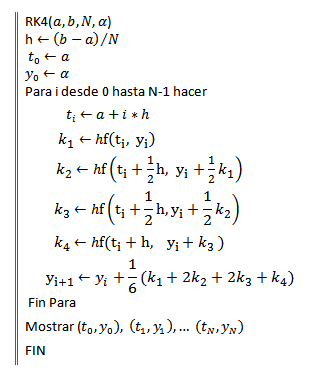
\includegraphics[width=0.50\textwidth]{alg_rk4}
% \caption{Figura-I.\label{fig: tahi}}
% }
% \end{figure}

.
\begin{definition}

\end{definition}

\begin{theorem}

\end{theorem}

\begin{corollary}
	aslkjdfkl;asjdfk;ljasd;lkfjal;ksjgklasjkgajsf
\end{corollary}

% no tocar por si hace falta despues pero esta bien feo
% {\footnotesize
% \begin{hangref}
% \item Banks, J., J. S. Carson, B. L. Nelson, and D. M. Nicol. 2000. \textit{Discrete-Event System Simulation}. 3rd ed. Upper Saddle River, New Jersey: Prentice-Hall, Inc.
% \end{hangref}
% }

\section*{Conclusiones}
Este estudio proporciona una comprensi\'on más profunda de las complejas interacciones entre los depredadores y sus presas en
los ecosistemas naturales. Los resultados obtenidos pueden ser \'utiles para predecir y manejar las poblaciones de presas y
depredadores en diferentes entornos y para comprender mejor los efectos del cambio clim\'atico y otros factores ambientales
en estas interacciones. FALTA Añadir una valoración de lo que usted ha aprendido con este trabajo, como valora la
posibilidad de que se pueda continuar esta línea de investigación.

\section*{F\'ORMULAS A UTILIZAR DESPU\'ES}
% aqui ya estan la mayoria de las formulas

\begin{equation} \label{JacobianoEstability}
	J\left(x^*, y^*, z^*\right)=\left[\begin{array}{ccc}
			\mathrm{r}-\frac{2 r x}{k}-\beta-\alpha z & 0                                                                  & -\alpha x                                        \\
			\beta                                     & -\frac{\eta \mathrm{z}}{y+m}+\frac{\eta y \mathrm{z}}{(y+m)^2}-\mu & -\frac{\eta \mathrm{y}}{y+m}                     \\
			\alpha_1 z                                & \frac{\eta_1 \mathrm{z}^2}{(y+m)^2}                                & 2 p z-\frac{2 \eta_1 \mathrm{z}}{y+m}+\alpha_1 x
		\end{array}\right]
\end{equation}

\begin{equation} \label{twoPreyonePredator_Falconi}
	\begin{gathered}
		\frac{d x_1}{d t}=r x_1\left(1-\frac{x_1}{K}\right)-\beta x_1-\frac{\beta_1 x_1 y}{1+m_1 x_1^2+n_1 x_2} \\
		\frac{d x_2}{d t}=\beta x_1-\frac{\beta_2 x_2 y}{1+m_2 x_1+n_2 x_2}-\mu_1 x_2                           \\
		\frac{d y}{d t}=\frac{\alpha_1 \beta_1 x_1 y}{1+m_1 x_1^2+n_1 x_2}+\frac{\alpha_2 \beta_2 x_2 y}{1+m_2 x_1+n_2 x_2}-\mu_2 y
	\end{gathered}
\end{equation}

\begin{equation} \label{Holling1y2_Abadi}
	\begin{gathered}
		\frac{d x_1}{d t}=r x_1\left(1-\frac{x_1}{K}\right)-\beta x_1-\alpha x_1 y \\
		\frac{d x_2}{d t}=\beta x_1-\frac{\varepsilon x_2 y}{1+m x_2}-\mu_1 x_2 \\
		\frac{d y}{d t}=\frac{\gamma \varepsilon x_2 y}{1+m x_2}-\mu_2 y
	\end{gathered}
\end{equation}

\begin{equation} \label{Holling1y2_Castellanos}
	\begin{gathered}
		\frac{d x}{d t}=\rho x\left(1-\frac{x}{k}\right)-a_1 x \\
		\frac{d y}{d t}=c a_1 x y-d y-\frac{a_2 y z}{y+b_2} \\
		\frac{d z}{d t}=\alpha z^2-\frac{\beta z^2}{y+b_2}
	\end{gathered}
\end{equation}

\begin{equation} \label{twoPreyonePredatorEDO}
	\begin{gathered}
		\frac{d x}{d t}=r x\left(1-\frac{x}{k}\right)-\beta x-\alpha x z \\
		\frac{d y}{d t}=\beta x-\frac{\eta y z}{y+m}-\mu y \\
		\frac{d z}{d t}=\alpha_1 x z+\rho z^2-\frac{\eta_1 y z}{y+m}
	\end{gathered}
\end{equation}

\begin{equation} \label{Characteristic000}
	\left|\begin{array}{ccc}
		(-1+r)-\lambda & 0            & 0         \\
		\beta          & -\mu-\lambda & 0         \\
		0              & 0            & 0-\lambda
	\end{array}\right|=0
\end{equation}

\begin{equation} \label{Equilibrium}
	\begin{aligned}
		 & \operatorname{det}\left(J\left(\frac{k(r-\beta)}{r}, \frac{\beta k(r-\beta)}{\mu r}, 0\right)-\lambda I\right)=0                            \\
		 & J\left(E_2\right)=\left|\begin{array}{ccc}
			                           (\beta-r)-\lambda & 0            & \frac{\alpha k(\beta-r)}{r}                                                      \\
			                           \beta             & -\mu-\lambda & \frac{\eta \beta k(\beta-r)}{r \mu\left(\frac{\beta k(r-\beta)}{\mu r}+m\right)} \\
			                           0                 & 0            & -\frac{\alpha_1 k(\beta-r)}{r}
		                           \end{array}\right|=0
	\end{aligned}
\end{equation}

\begin{equation} \label{CharacteristicPolynomial}
	J\left(x^*, y^*, z^*\right)=\left[\begin{array}{ccc}
			\mathrm{r}-\frac{2 r x^*}{k}-\beta-\alpha z^* & 0                                                                   & -\alpha x^*                                     \\
			\beta                                         & -\frac{\eta z^*}{y^*+m}+\frac{\eta y z^*}{\left(y^*+m\right)^2}-\mu & -\frac{\eta y^*}{y^*+m}                         \\
			\alpha_1 z^*                                  & \frac{\eta_1 z^{* 2}}{\left(y^*+m\right)^2}                         & 2 p z^*-\frac{2 \eta_1 z^*}{y^*+m}+\alpha_1 x^*
		\end{array}\right]
\end{equation}

\defbibheading{Referencias}{\section*{Referencias}}
\defbibheading{Bibliografía}{\section*{Bibliografía}}

\printbibliography[heading=Referencias, type=article]
\renewcommand{\theenumiv}{}
\DeclareFieldFormat{labelnumberwidth}{}
\printbibliography[heading=Bibliografía, type=book, resetnumbers=true]
\nocite{edwards_differential_2008}



\section*{Agradeciemientos}
Agradecemos a nuestros queridos profesores por lograr que entendieramos de que van las ecuaciones diferenciales

\appendix

\section{Anexos} \label{app:quadratic}

\begin{equation} \label{eq:quadraticsol}
	x = \frac{-b \pm \sqrt{b^2-4ac}}{2a} \mbox{ si } a \ne 0.
\end{equation}

\end{document}

